\section{Results and sensitivity analysis}\label{results}

% TODO: verbale beschreibung des modells ==> extrem hineingehen und deckeln und stattdessen in den investment grant. hinein führen zu den ergebnissen. energiepolitik. 

\begin{figure}[h]
	\centering
	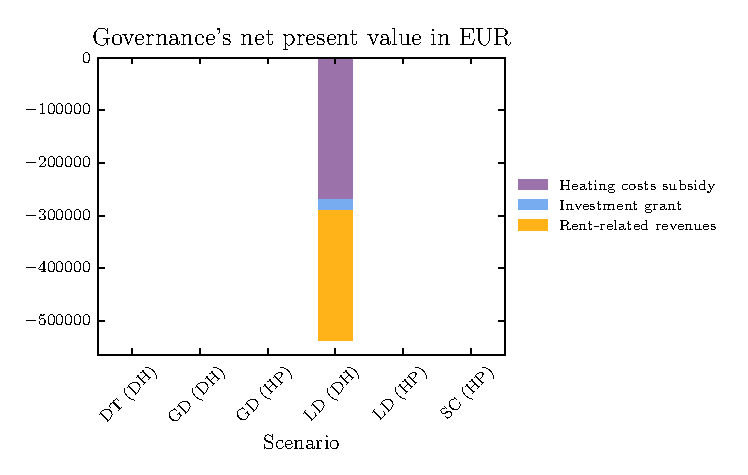
\includegraphics[width=1\linewidth]{figures/4_Results/fig_npv_comparison/net_present_value.eps}
	\caption{}
	\label{fig:npv_comparison}
\end{figure}

\begin{figure}[h]
	\centering
	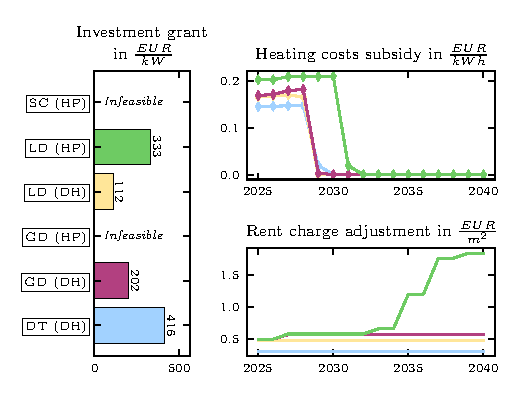
\includegraphics[width=1\linewidth]{figures/4_Results/fig_rent_subsidy_development/price_dev.eps}
	\caption{}
	\label{fig:sub_rent_dev}
\end{figure}

% TODO Einpreisen der Mieterwechsel (Leerstand) in "Interest rate" des Landlords

% TODO Vergleich zwischen Government wo Gebäudesanierung voraussetzung ist und einmal ohne Gebäudesanierung - Demand seitige Anpassung
% TODO Gegenüberstellen: Einmal vergisst Staat auf Gebäudesanierung und einmal nicht, was ist das Delta an NPV. 

% TODO: Eventuell ist Modell dann nicht mehr Lösbar und was müsste die CO2 Aufteilung sein, damit es eine Lösung gibt. 